\chapter[Literature review]{Literature review}

\section{Introduction}
Most contemporary nuclear reactor physics software is unable to perform depletion calculations in an online reprocessing regime. Furthermore, no established tool for liquid-fueled \gls{MSR} neutronics and fuel cycle evaluation exist, except internally developed tools from universities and research institutions can approximate online refueling. The foundation for these tools was based on early \gls{MSR} simulation methods at \gls{ORNL}, which integrated neutronic and fuel cycle codes (i.e., Reactor 
Optimum Design (ROD) \cite{bauman_rod_1971}) into operational plant tools (i.e., 
Multiregion Processing Plant (MRPP) \cite{kee_mrpp_1976}) for \gls{MSR} and 
reprocessing system design. Based on 
this approach, recent tools from universities and research institutions can
approximate online refueling \cite{serp_molten_2014-1}. A summary of recent
efforts is listed in table~\ref{tab:fs_codes}.
\begin{table}[ht!]
\caption{Tools and methods for liquid-fueled \glspl{MSR} fuel salt depletion analysis.}
\begin{tabularx}{\textwidth}{ m | b | x } 
\hline Neutronic code    & \qquad Authors & Spectrum   \\
\hline
\gls{MCNP}/REM \cite{noauthor_mcnp_2004,heuer_simulation_2010}  & Doligez 
\emph{et al.}, 2014; Heuer \emph{et al.}, 2014  
\cite{doligez_coupled_2014,heuer_towards_2014}    & fast \\
\hline
ERANOS \cite{ruggieri_eranos_2006}  & Fiorina \emph{et al.}, 2013 
\cite{fiorina_investigation_2013}            & fast \\
\hline
KENO-IV/ORIGEN \cite{goluoglu_monte_2011,gauld_isotopic_2011}     & Sheu 
\emph{et al.}, 2013 \cite{sheu_depletion_2013} & fast \\
\hline
SERPENT2 \cite{leppanen_serpent_2015}  & Aufiero \emph{et al.}, 2013 
\cite{aufiero_extended_2013}; Ashraf \emph{et al.}, 2018 \cite{ashraf_nuclear_2018} & fast \\
\hline
DIF3D \cite{derstine_dif3d_1984} & Zhou \emph{et al.}, 2018 
\cite{zhou_fuel_2018-1} & thermal/ fast \\
\hline
\gls{MCNP}/REM  & Nuttin \emph{et al.} \cite{nuttin_potential_2005}&thermal  \\ 
\hline
MCODE/ORIGEN2 \cite{xu_mcode_2008,croff_users_1980}      & Ahmad \emph{et al.}, 
2015 \cite{ahmad_neutronics_2015}   & thermal  \\
\hline
OpenMC/ORIGEN-S \cite{romano_openmc_2015,rearden_scale_2018}  & de Lanversin \emph{et al.}, 
2017 \cite{de_troullioud_de_lanversin_toward_2017}   & thermal  \\
\hline
\gls{MCNP}6/CINDER90 \cite{goorley_mcnp6_2013}     & Park \emph{et al.}, 2015; 
Jeong \emph{et al.}, 2016 \cite{park_whole_2015, jeong_equilibrium_2016}& 
thermal\\
\hline
SCALE/TRITON \cite{bowman_scale_2011,powers_new_2013}    & Powers \emph{et al.}, 
2014; Betzler \emph{et al.}, 2017; Li \emph{et al.}, 2018
\cite{powers_new_2013,powers_inventory_2014,betzler_molten_2017, li_optimization_2018} & thermal/ fast\\
\hline
SERPENT2     & Rykhlevskii \emph{et al.}, 2017-2019 \cite{rykhlevskii_online_2017, rykhlevskii_full-core_2017, rykhlevskii_advanced_2018,rykhlevskii_modeling_2019} & 
thermal\\
\hline
\end{tabularx}
  \label{tab:fs_codes}
\end{table}
\FloatBarrier

References \cite{li_optimization_2018,de_troullioud_de_lanversin_toward_2017,doligez_coupled_2014,
heuer_towards_2014, sheu_depletion_2013, aufiero_extended_2013} provide some form of reactivity control, 
and methods \cite{doligez_coupled_2014,heuer_towards_2014,aufiero_extended_2013,ahmad_neutronics_2015, 
park_whole_2015,jeong_equilibrium_2016,rykhlevskii_modeling_2019,nuttin_potential_2005} use a set of all nuclides in depletion calculations. 

\section{Batch-wise online reprocessing approach}
Many liquid-fueled \gls{MSR} designs rely on online fuel processing in which  
material moves to and from the core continuously or at specific time steps 
(batch-wise). In the batch-wise approach, the burn-up simulation stops at a given 
time and restarts with a new liquid fuel composition (after removal of discarded 
materials and addition of fissile/fertile materials). \gls{ORNL} researchers 
have developed ChemTriton, a Python-based script for SCALE/TRITON which uses the 
batch-wise approach to simulate a continuous reprocessing and refill for either single 
or multiple fluid designs. ChemTriton models salt 
treatment, separations, discharge, and refill using a unit-cell \gls{MSR} 
SCALE/TRITON depletion simulation over small time steps to simulate continuous 
reprocessing and deplete the fuel salt \cite{powers_new_2013}. Methods listed in 
references \cite{zhou_fuel_2018-1,sheu_depletion_2013,park_whole_2015,jeong_equilibrium_2016, powers_inventory_2014,betzler_molten_2017,rykhlevskii_modeling_2019} 
as also employ a batch-wise approach. This approach has a few disadvantages. First, 
this method assumes that material transfer from the reactor primary loop to the reprocessing 
plant is discrete and instantaneous. In reality, some small fraction of fuel salt \textbf{continuously} flowing to reprocessing plant and approximately the same 
\textbf{continuous} material flow returning back to keep mass balance in a 
primary loop. Second, this approach assumes that material accumulation in the core 
during the time between separations or feeds does not affect reactor physics which 
is not true for relatively long (few days) depletion simulation time steps. These assumptions for simulation of the nonstop online reprocessing process tends to
 misrepresent depleted material composition obtained from simulation.

\section{Continuous online reprocessing approach}
Accounting for continuous removal or addition presents a greater challenge since it 
requires adding a term to the Bateman equations. In SCALE/TRITON, ORIGEN \cite{gauld_isotopic_2011} solves a set of Bateman equations using one-group averaged fluxes and cross-sections obtained from a transport calculation. Bateman equations that describe the rate of change of the isotopes due to neutron induced reactions and decay
processes could be written in this form \cite{aufiero_extended_2013}:

\begin{align}
        \frac{dN_i}{dt} &= \bar{\Phi}\sum\limits_{j}N_{j}\sigma_{j \rightarrow 		i} - \bar{\Phi}\sum\limits_{j}N_{i}\sigma_{i \rightarrow j} + \sum					\limits_{j}	N_{j}\lambda_{j}b_{j \rightarrow i} - N_{i}\lambda_{i}
\label{eq:bateman}
	\intertext{where} 
	N_i &= \mbox{number density of isotope i} \\
	N_j &= \mbox{number density of isotope j} \\
	\bar{\Phi} &= \mbox {average in the space and energy neutron flux} \\
	\sigma_{j \rightarrow i} &= \mbox{microscopic one-group transmutation cross section} \\
	\lambda_i &= \mbox{decay constant of nuclide i} \\
	\lambda_j &= \mbox{decay constant of nuclide j} \\
	b_{j \to i} &= \mbox{branching fractions of radioactive decay from nuclide j}
\end{align}

The four terms on the right-hand side of the equation represent (1) the production rate of nuclide $i$ from irradiation, (2) the loss rate of nuclide $i$ due to irradiation, (3) the decay rate of nuclide $j$ into nuclide $i$, and (4) the loss rate of nuclide $i$ due to decay. Mentioned earlier deterministic codes SCALE/TRITON and Monte Carlo codes MCNP, Shift, KENO-VI do not support non-zero removal or feeds rates for depletion simulations.

Online fuel reprocessing can be explicitly introduced in the system of equations by adding effective decay and transmutation terms for the various nuclides. Fuel refill during fuel salt composition evolution calculations could be taken into account by
adding a gain term on the right-hand side of the Bateman equation:
\begin{align} 
\bar{\Phi}\sum\limits_{k=^{235}U}N_{k}\sigma_{k,c}  \label{eq:feed_term}
\end{align}
where $\sigma_{k,c}$ is the one-group capture cross section of feed isotope (e.g. uranium-235).

The removal of fission products and protactinium is achieved by adding an explicit decay term to the Bateman equations. For the generic fission product, $l$, loss term can be added:
\begin{align} 
- N_{l}\lambda_{l,removal}  \label{eq:rem_term}
\end{align}
where $\lambda_{l,removal}$ is the effective removal time constant of the particular chemical species. 

Fiorina \emph{et al.} simulated 
\gls{MSFR} depletion with continuous fuel salt reprocessing via introducing 
``reprocessing'' time constants into the ERANOS transport code 
\cite{fiorina_investigation_2013}. Similar approach used Nuttin \emph{et al.} to 
simulate online reprocessing with Monte Carlo MCNP code for \gls{MSBR}-like reference 
system with $^{232}$Th/$^{233}$U fuel \cite{nuttin_potential_2005}.
Same concept is adopted to model continuous feeds and extractions using the MCNP transport code listed in references \cite{doligez_coupled_2014,heuer_towards_2014}. 

This approach was recently implemented as a purpose-made extension within the continuous-energy Monte Carlo reactor physics and burn-up code SERPENT \cite{aufiero_extended_2013} 
using a described earlier methodology by explicitly introducing 
continuous reprocessing in the system of Bateman equations and adding effective 
decay and transmutation terms for each nuclide 
\cite{aufiero_extended_2013}. This was employed to study the material isotopic evolution of the \gls{MSFR}\cite{aufiero_extended_2013}. The developed extension directly 
accounts for the effects of online fuel 
reprocessing on depletion calculations and features a reactivity control 
algorithm. The extended version of SERPENT2 was assessed against a dedicated 
version of the deterministic ERANOS-based EQL3D procedure in
\cite{ruggieri_eranos_2006, fiorina_investigation_2013} and adopted to analyze 
the \gls{MSFR} fuel salt isotopic evolution. In addition, the latest SCALE release 
will also have the same functionality using truly continuous removals \cite{betzler_implementation_2017}. 

Nuttin \emph{et al.} broke up the reactor core geometry into three \gls{MCNP} cells: 
one for salt channels, one for the salt plena above and below the core, and a 
third cell for the annulus. Consequently, the two-region reactor core was 
approximated by one region with averaged fuel/moderator ratio 
\cite{nuttin_potential_2005}.  Powers \emph{et 
al.}, Betzler \emph{et al.}, and Jeong \emph{et al.} 
\cite{powers_new_2013,powers_inventory_2014,betzler_modeling_2016, 
betzler_molten_2017, jeong_development_2014, jeong_equilibrium_2016} used a 
similar simplified unit-cell models. This approach 
misrepresents the two-region breeder reactor concept. The unit-cell or one-region 
models may produce reliable results for homogeneous reactor cores (i.e. 
\gls{MSFR}, \gls{MOSART}) or for one-region single-fluid reactor designs (i.e. 
\gls{MSRE}). However, many reactor concepts with sophisticated geometry (e.g. 
two-region \gls{MSBR}, \gls{TAP} \gls{MSR} with irregular moderator pattern) must 
be simulated using a whole-core model to accurately capture different neutron 
transport characteristics in the 
different regions of the core. Therefore, online reprocessing tools and reactor 
physics codes should be tested using high-precision full-core reactor core models.

\section{Extraction efficiency}
References \cite{rykhlevskii_modeling_2019, li_optimization_2018, de_troullioud_de_lanversin_toward_2017, park_whole_2015, sheu_depletion_2013} assumed extraction efficiency for all isotopes equal 100\% (e.g. 100\% of mass of target isotopes removed within the ``cycle times''\footnote{ The \gls{MSBR} program defined a ``cycle time" as the amount of 
time required to reprocess entire salt ($T_r$) \cite{robertson_conceptual_1971}.}). 
Nuttin \emph{et al.} introduced separation efficiency ($\epsilon_e$) using following 
equation \cite{nuttin_potential_2005}
\begin{align}
dN_e = N_{e, 0} \frac{dt}{T_r} \epsilon_e
\end{align}
where $dN_e$ is extracted amount of element $e$; $N_{e, 0}$ is initial inventory 
of the element $e$,; $dt$ is time interval; $T_r$ is time needed to reprocess 
entire salt (cycle time). Integration of both part of this equation leads to 
following expression for element $e$ amount after extraction:
\begin{align}
N_{e, 1} = N_{e, 0} e^{\frac{\epsilon_e}{T_r}t}
\end{align}
For the simplified case when efficiency selected equal 100\%, effective removal 
time constant 
($\lambda_e$) for element $e$ can be estimated as follows:
\begin{align} 
\lambda_e = \epsilon_e / T_r  \label{eq:100_lam}
\end{align}
For the case with realistic separation efficiency (e.g. 99\% for uranium extraction) effective removal time constant for element $e$ can be expressed as
 \cite{nuttin_potential_2005}:
\begin{align}  
\lambda_e = \frac{ln |1-\epsilon_e|}{T_r} \label{eq:real_lam}
\end{align}
The equation \ref{eq:real_lam} is exponential extrapolation and has been used to 
estimate removal constant for 
extraction term in the Bateman equations (\ref{eq:rem_term}) in references \cite{nuttin_potential_2005, betzler_implementation_2017, doligez_coupled_2014}.

\section{Online reprocessing tool simulation flow charts}
Liquid-fueled systems present a challenge to existing neutron transport and depletion tools, which are typically designed to simulate solid-fueled reactors. To handle the material flows and online removal and feed of \gls{MSR} researchers developed in-house 
tools which usually built on top of existing neutron transport and depletion code. Figure~\ref{fig:typical_flow_chart} demonstrates typical flow charts for batch-wise 
(references \cite{betzler_molten_2017, li_optimization_2018, 
rykhlevskii_modeling_2019, zhou_fuel_2018-1,sheu_depletion_2013,park_whole_2015}) and 
online reprocessing (references \cite{heuer_simulation_2010, doligez_coupled_2014,  heuer_towards_2014, fiorina_investigation_2013, nuttin_potential_2005, aufiero_extended_2013, de_troullioud_de_lanversin_toward_2017}) codes. Almost all of 
existing codes representing chemical reprocessing plant as ``single box'' 
model (orange ellipses on figure~\ref{fig:typical_flow_chart}) which removes target 
elements all at once with constant efficiency. Typical inputs and outputs for this 
``single box'' model are vectors of elements and extraction efficiencies and can be 
expressed as follows:
\begin{equation}
\begin{bmatrix}
N^{in}_{element \: 1} \\ N^{in}_{element \: i} \\ \vdots \\
\end{bmatrix} 
\times
\begin{bmatrix}
\epsilon_{element \: 1} \\ \epsilon_{element \: i} \\ \vdots \\
\end{bmatrix} =
\begin{bmatrix}
N^{out}_{element \: 1} \\ N^{out}_{element \: i} \\ \vdots \\
\end{bmatrix}
\end{equation}
where $N^{in/out}_i$ is the number of atoms of $i^{th}$ element and $\epsilon_i$ is the 
extraction efficiency for $i^{th}$ element. There are few issues with simplified 
``single box'' model: 
\begin{enumerate}
	\item Current research efforts assumed than separation 
efficiency vector is not changing with time and does not depend from reactor 
operational parameters (separation efficiency might changes with temperature, 
power level, current fuel salt isotope composition, etc).
	\item Fuel salt during reprocessing plant undergo not a single but many 
	separate processes 
	(e.g. He bubbling quickly extracting the gaseous \glspl{FP}, nickel mesh filter 
	extracting noble  and  semi-noble  metal  solid  \glspl{FP}, etc). Some of 
	these processes can be done concurrently but many are sequential.
	\item Ignoring decaying of radioactive nuclides during processing on 
	the reprocessing plant (chemical separation is not instantaneous process) 
	especially for process sequences. 
	\item Each chemical process is related with chemical facility which has 
	limited volume (for batch process) and/or capacity (for continuous process). 
	Moreover, separation efficiency of the facility toughly related material flow 
	rate (higher mass flow rate leads to lower separation efficiency \cite{briggs_molten-salt_1969}).
\end{enumerate}

\begin{figure}[hbp!] % replace 't' with 'b' to \centering
  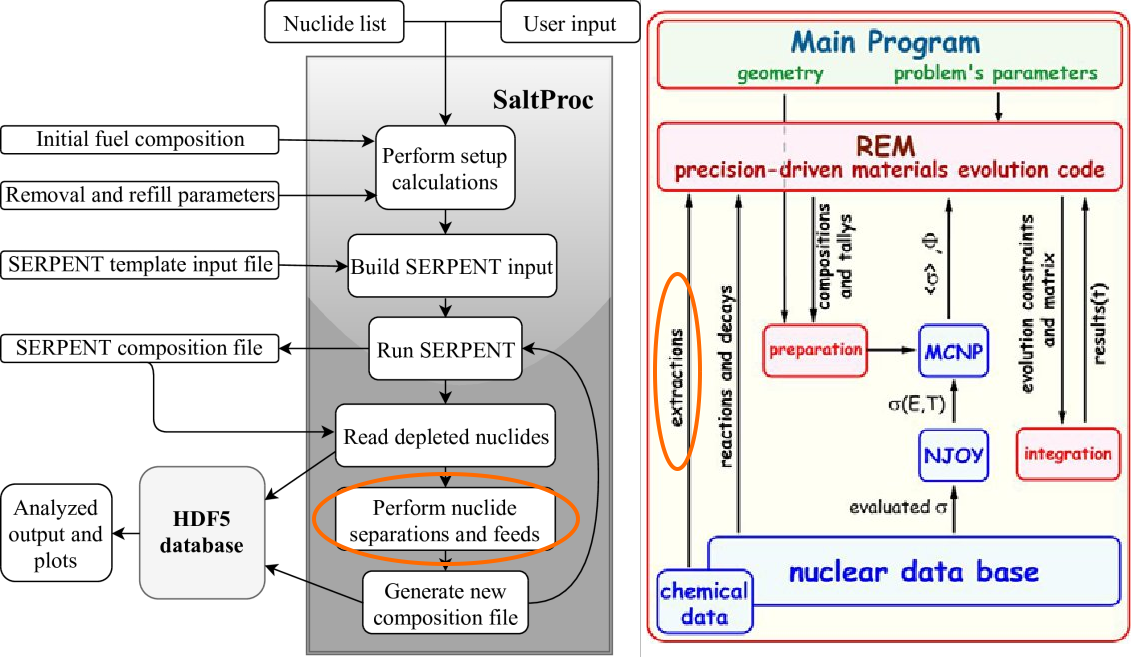
\includegraphics[width=\textwidth]{typical_flow_chart.png}
  \caption{Typical flow charts of online reprocessing simulation tool:
  batch-wise tool SaltProc (uses SERPENT2 for neutron transport and 
  depeletion) \cite{rykhlevskii_modeling_2019}
   (left) and continuous  REM (uses MCNP as transport code) 
   \cite{heuer_simulation_2010} (right).} 
  \label{fig:typical_flow_chart}
\end{figure}

For realistic simulation ``single box'' with only separation efficiency as parameter
 should be substituted with different boxes each representing particular unit of
separation equipment. Simon \emph{et al.} made an effort to develop reprocessing code for realistic \gls{MSBR} reprocessing plant simulation 
which based on chemistry models \cite{simon_-line_2008}. The code represents 2 simple separation processes: (1)  protactinium 
extraction by reductive salt-metal extraction in a bismuth medium (original 
\gls{MSBR} method proposed by \gls{ORNL} \cite{whatley_engineering_1970-1}), and (2) 
lanthanides extraction based on 2 steps recovery process:  the reduction of 
lanthanides by lithium from the fluoride fuel salt to liquid bismuth, then the 
oxidation of lanthanides from liquid bismuth to a lithium chloride salt. Simon and 
colleagues applied this code to \gls{MSBR}-like reactor design and obtained realistic 
correlations for protactinium and lanthanides extraction efficiencies. Those 
correlations involved mass flow rates for the salt and liquid metal (Bi), 
distribution coefficient between fluoride salt and Bi-Li-Th, interfacial areas 
between fluoride salt and Bi-Li-Th, and mass transfer coefficient through the 
interface. Unfortunately, this research effort only modeled reprocessing plant 
and does not coupled with a neutronics code to simulate fuel salt depletion in 
the reactor core. Online reprocessing 
tool which simulates fuel salt depletion in the core and realistically models 
reprocessing plant would allows modeling of the comprehensive behaviour of 
Molten Salt liquid-fueled system, including, in a coupled manner, both the 
design of the core and the optimized reprocessing scheme effects.
